% Copyright © 2013 Martin Ueding <dev@martin-ueding.de>

% Copyright © 2012-2013 Martin Ueding <dev@martin-ueding.de>

% This is my general purpose LaTeX header file for writing German documents.
% Ideally, you include this using a simple ``% Copyright © 2012-2013 Martin Ueding <dev@martin-ueding.de>

% This is my general purpose LaTeX header file for writing German documents.
% Ideally, you include this using a simple ``% Copyright © 2012-2013 Martin Ueding <dev@martin-ueding.de>

% This is my general purpose LaTeX header file for writing German documents.
% Ideally, you include this using a simple ``\input{header.tex}`` in your main
% document and start with ``\title`` and ``\begin{document}`` afterwards.

% If you need to add additional packages, I recommend not doing this in this
% file, but in your main document. That way, you can just drop in a new
% ``header.tex`` and get all the new commands without having to merge manually.

% Since this file encorporates a CC-BY-SA fragment, this whole files is
% licensed under the CC-BY-SA license.

\documentclass[11pt, ngerman, fleqn, DIV=15, headinclude, BCOR=2cm]{scrartcl}

\usepackage{graphicx}

% Environment to quote the problem. Currently, this is just a new name for the
% quote environment.
\newenvironment{problem}{\begin{quote}\textsf{\textbf{Aufgabenstellung:}}\quad}{\end{quote}}

\setkomafont{caption}{\sf}
\setkomafont{captionlabel}{\usekomafont{caption}}

%%%%%%%%%%%%%%%%%%%%%%%%%%%%%%%%%%%%%%%%%%%%%%%%%%%%%%%%%%%%%%%%%%%%%%%%%%%%%%%
%                                Locale, date                                 %
%%%%%%%%%%%%%%%%%%%%%%%%%%%%%%%%%%%%%%%%%%%%%%%%%%%%%%%%%%%%%%%%%%%%%%%%%%%%%%%

\usepackage{babel}
\usepackage[iso]{isodate}

%%%%%%%%%%%%%%%%%%%%%%%%%%%%%%%%%%%%%%%%%%%%%%%%%%%%%%%%%%%%%%%%%%%%%%%%%%%%%%%
%                          Margins and other spacing                          %
%%%%%%%%%%%%%%%%%%%%%%%%%%%%%%%%%%%%%%%%%%%%%%%%%%%%%%%%%%%%%%%%%%%%%%%%%%%%%%%

\usepackage[parfill]{parskip}
\usepackage{setspace}
\usepackage[activate]{microtype}

\setlength{\columnsep}{2cm}

%%%%%%%%%%%%%%%%%%%%%%%%%%%%%%%%%%%%%%%%%%%%%%%%%%%%%%%%%%%%%%%%%%%%%%%%%%%%%%%
%                                    Color                                    %
%%%%%%%%%%%%%%%%%%%%%%%%%%%%%%%%%%%%%%%%%%%%%%%%%%%%%%%%%%%%%%%%%%%%%%%%%%%%%%%

\usepackage[usenames, dvipsnames]{xcolor}

\colorlet{darkred}{red!70!black}
\colorlet{darkblue}{blue!70!black}
\colorlet{darkgreen}{green!40!black}

%%%%%%%%%%%%%%%%%%%%%%%%%%%%%%%%%%%%%%%%%%%%%%%%%%%%%%%%%%%%%%%%%%%%%%%%%%%%%%%
%                         Font and font like settings                         %
%%%%%%%%%%%%%%%%%%%%%%%%%%%%%%%%%%%%%%%%%%%%%%%%%%%%%%%%%%%%%%%%%%%%%%%%%%%%%%%

% This replaces all fonts with Bitstream Charter, Bitstream Vera Sans and
% Bitstream Vera Mono. Math will be rendered in Charter.
\usepackage[charter, greekuppercase=italicized]{mathdesign}
\usepackage{beramono}
\usepackage{berasans}

% Bold, sans-serif tensors. This fragment is taken from “egreg” from
% http://tex.stackexchange.com/a/82747/8945 and licensed under `CC-BY-SA
% <https://creativecommons.org/licenses/by-sa/3.0/>`_.
\usepackage{bm}
\DeclareMathAlphabet{\mathsfit}{\encodingdefault}{\sfdefault}{m}{sl}
\SetMathAlphabet{\mathsfit}{bold}{\encodingdefault}{\sfdefault}{bx}{sl}
\newcommand{\tens}[1]{\bm{\mathsfit{#1}}}

% Bold vectors.
\renewcommand{\vec}[1]{\boldsymbol{#1}}

%%%%%%%%%%%%%%%%%%%%%%%%%%%%%%%%%%%%%%%%%%%%%%%%%%%%%%%%%%%%%%%%%%%%%%%%%%%%%%%
%                               Input encoding                                %
%%%%%%%%%%%%%%%%%%%%%%%%%%%%%%%%%%%%%%%%%%%%%%%%%%%%%%%%%%%%%%%%%%%%%%%%%%%%%%%

\usepackage[T1]{fontenc}
\usepackage[utf8]{inputenc}

%%%%%%%%%%%%%%%%%%%%%%%%%%%%%%%%%%%%%%%%%%%%%%%%%%%%%%%%%%%%%%%%%%%%%%%%%%%%%%%
%                         Hyperrefs and PDF metadata                          %
%%%%%%%%%%%%%%%%%%%%%%%%%%%%%%%%%%%%%%%%%%%%%%%%%%%%%%%%%%%%%%%%%%%%%%%%%%%%%%%

\usepackage{hyperref}
\usepackage{lastpage}

% This sets the author in the properties of the PDF as well. If you want to
% change it, just override it with another ``\hypersetup`` call.
\hypersetup{
	breaklinks=false,
	citecolor=darkgreen,
	colorlinks=true,
	linkcolor=darkblue,
	menucolor=black,
	pdfauthor={Martin Ueding},
	urlcolor=darkblue,
}

%%%%%%%%%%%%%%%%%%%%%%%%%%%%%%%%%%%%%%%%%%%%%%%%%%%%%%%%%%%%%%%%%%%%%%%%%%%%%%%
%                               Math Operators                                %
%%%%%%%%%%%%%%%%%%%%%%%%%%%%%%%%%%%%%%%%%%%%%%%%%%%%%%%%%%%%%%%%%%%%%%%%%%%%%%%

% AMS environments like ``align`` and theorems like ``proof``.
\usepackage{amsmath}
\usepackage{amsthm}

% Common math constructs like partial derivatives.
\usepackage{commath}

% Physical units.
\usepackage[output-decimal-marker={,}]{siunitx}

% Since I use mathdesign with italic uppercase greek characters, the Ohm unit will be displayed with an italic Ω by default. Units have to be roman, so this forces it the right way.
\DeclareSIUnit{\ohm}{$\Omegaup$}
\DeclareSIUnit{\division}{DIV}

% Word like operators.
\DeclareMathOperator{\acosh}{arcosh}
\DeclareMathOperator{\arcosh}{arcosh}
\DeclareMathOperator{\arcsinh}{arsinh}
\DeclareMathOperator{\arsinh}{arsinh}
\DeclareMathOperator{\asinh}{arsinh}
\DeclareMathOperator{\card}{card}
\DeclareMathOperator{\csch}{cshs}
\DeclareMathOperator{\diam}{diam}
\DeclareMathOperator{\sech}{sech}
\renewcommand{\Im}{\mathop{{}\mathrm{Im}}\nolimits}
\renewcommand{\Re}{\mathop{{}\mathrm{Re}}\nolimits}

% Fourier transform.
\DeclareMathOperator{\fourier}{\ensuremath{\mathcal{F}}}

% Roman versions of “e” and “i” to serve as Euler's number and the imaginary
% constant.
\newcommand{\ee}{\eup}
\newcommand{\eup}{\mathrm e}
\newcommand{\ii}{\iup}
\newcommand{\iup}{\mathrm i}

% Symbols for the various mathematical fields (natural numbers, integers,
% rational numbers, real numbers, complex numbers).
\newcommand{\C}{\ensuremath{\mathbb C}}
\newcommand{\N}{\ensuremath{\mathbb N}}
\newcommand{\Q}{\ensuremath{\mathbb Q}}
\newcommand{\R}{\ensuremath{\mathbb R}}
\newcommand{\Z}{\ensuremath{\mathbb Z}}

% Shape like operators.
\DeclareMathOperator{\dalambert}{\Box}
\DeclareMathOperator{\laplace}{\bigtriangleup}
\newcommand{\curl}{\vnabla \times}
\newcommand{\divergence}[1]{\inner{\vnabla}{#1}}
\newcommand{\vnabla}{\vec \nabla}

\newcommand{\half}{\frac 12}

% Unit vector (German „Einheitsvektor“).
\newcommand{\ev}{\hat{\vec e}}

% Scientific notation for large numbers.
\newcommand{\e}[1]{\cdot 10^{#1}}

% Mathematician's notation for the inner (scalar, dot) product.
\newcommand{\bracket}[1]{\left\langle #1 \right\rangle}
\newcommand{\inner}[2]{\bracket{#1, #2}}

% Placeholders.
\newcommand{\emesswert}{\del{\messwert \pm \messwert}}
\newcommand{\fehlt}{\textcolor{darkred}{Hier fehlen noch Inhalte.}}
\newcommand{\messwert}{\textcolor{blue}{\square}}
\newcommand{\punkte}{\phantom{xxxxx}}
\newcommand{\punktevon}[1]{\begin{flushright}/ #1\end{flushright}}

% Separator for equations on a single line.
\newcommand{\eqnsep}{,\quad}

% Quantum Mechanics
\usepackage{braket}

%%%%%%%%%%%%%%%%%%%%%%%%%%%%%%%%%%%%%%%%%%%%%%%%%%%%%%%%%%%%%%%%%%%%%%%%%%%%%%%
%                                  Headings                                   %
%%%%%%%%%%%%%%%%%%%%%%%%%%%%%%%%%%%%%%%%%%%%%%%%%%%%%%%%%%%%%%%%%%%%%%%%%%%%%%%

% This will set fancy headings to the top of the page. The page number will be
% accompanied by the total number of pages. That way, you will know if any page
% is missing.
%
% If you do not want this for your document, you can just use
% ``\pagestyle{plain}``.

\usepackage{scrpage2}

\pagestyle{scrheadings}
\automark{section}
\cfoot{\footnotesize{Seite \thepage\ / \pageref{LastPage}}}
\chead{}
\ihead{}
\ohead{\rightmark}
\setheadsepline{.4pt}

%%%%%%%%%%%%%%%%%%%%%%%%%%%%%%%%%%%%%%%%%%%%%%%%%%%%%%%%%%%%%%%%%%%%%%%%%%%%%%%
%                            Bibliography (BibTeX)                            %
%%%%%%%%%%%%%%%%%%%%%%%%%%%%%%%%%%%%%%%%%%%%%%%%%%%%%%%%%%%%%%%%%%%%%%%%%%%%%%%

\newcommand{\bibliographyfile}{../../zentrale_BibTeX/Central}
\bibliographystyle{apalike2}

%%%%%%%%%%%%%%%%%%%%%%%%%%%%%%%%%%%%%%%%%%%%%%%%%%%%%%%%%%%%%%%%%%%%%%%%%%%%%%%
%                                Abbreviations                                %
%%%%%%%%%%%%%%%%%%%%%%%%%%%%%%%%%%%%%%%%%%%%%%%%%%%%%%%%%%%%%%%%%%%%%%%%%%%%%%%

\newcommand{\dhabk}{\mbox{d.\,h.}}

%%%%%%%%%%%%%%%%%%%%%%%%%%%%%%%%%%%%%%%%%%%%%%%%%%%%%%%%%%%%%%%%%%%%%%%%%%%%%%%
%                                  Licences                                   %
%%%%%%%%%%%%%%%%%%%%%%%%%%%%%%%%%%%%%%%%%%%%%%%%%%%%%%%%%%%%%%%%%%%%%%%%%%%%%%%

\usepackage{ccicons}

\newcommand{\ccbysadetext}{%
	\begin{small}
		Dieses Werk bzw. Inhalt steht unter einer
		\href{http://creativecommons.org/licenses/by-sa/3.0/deed.de}{%
			Creative Commons Namensnennung - Weitergabe unter gleichen
		Bedingungen 3.0 Unported Lizenz}.
	\end{small}
}

\newcommand{\ccbysadetitle}{%
	Lizenz: \href{http://creativecommons.org/licenses/by-sa/3.0/deed.de}
	{CC-BY-SA 3.0 \ccbysa}
}
`` in your main
% document and start with ``\title`` and ``\begin{document}`` afterwards.

% If you need to add additional packages, I recommend not doing this in this
% file, but in your main document. That way, you can just drop in a new
% ``header.tex`` and get all the new commands without having to merge manually.

% Since this file encorporates a CC-BY-SA fragment, this whole files is
% licensed under the CC-BY-SA license.

\documentclass[11pt, ngerman, fleqn, DIV=15, headinclude, BCOR=2cm]{scrartcl}

\usepackage{graphicx}

% Environment to quote the problem. Currently, this is just a new name for the
% quote environment.
\newenvironment{problem}{\begin{quote}\textsf{\textbf{Aufgabenstellung:}}\quad}{\end{quote}}

\setkomafont{caption}{\sf}
\setkomafont{captionlabel}{\usekomafont{caption}}

%%%%%%%%%%%%%%%%%%%%%%%%%%%%%%%%%%%%%%%%%%%%%%%%%%%%%%%%%%%%%%%%%%%%%%%%%%%%%%%
%                                Locale, date                                 %
%%%%%%%%%%%%%%%%%%%%%%%%%%%%%%%%%%%%%%%%%%%%%%%%%%%%%%%%%%%%%%%%%%%%%%%%%%%%%%%

\usepackage{babel}
\usepackage[iso]{isodate}

%%%%%%%%%%%%%%%%%%%%%%%%%%%%%%%%%%%%%%%%%%%%%%%%%%%%%%%%%%%%%%%%%%%%%%%%%%%%%%%
%                          Margins and other spacing                          %
%%%%%%%%%%%%%%%%%%%%%%%%%%%%%%%%%%%%%%%%%%%%%%%%%%%%%%%%%%%%%%%%%%%%%%%%%%%%%%%

\usepackage[parfill]{parskip}
\usepackage{setspace}
\usepackage[activate]{microtype}

\setlength{\columnsep}{2cm}

%%%%%%%%%%%%%%%%%%%%%%%%%%%%%%%%%%%%%%%%%%%%%%%%%%%%%%%%%%%%%%%%%%%%%%%%%%%%%%%
%                                    Color                                    %
%%%%%%%%%%%%%%%%%%%%%%%%%%%%%%%%%%%%%%%%%%%%%%%%%%%%%%%%%%%%%%%%%%%%%%%%%%%%%%%

\usepackage[usenames, dvipsnames]{xcolor}

\colorlet{darkred}{red!70!black}
\colorlet{darkblue}{blue!70!black}
\colorlet{darkgreen}{green!40!black}

%%%%%%%%%%%%%%%%%%%%%%%%%%%%%%%%%%%%%%%%%%%%%%%%%%%%%%%%%%%%%%%%%%%%%%%%%%%%%%%
%                         Font and font like settings                         %
%%%%%%%%%%%%%%%%%%%%%%%%%%%%%%%%%%%%%%%%%%%%%%%%%%%%%%%%%%%%%%%%%%%%%%%%%%%%%%%

% This replaces all fonts with Bitstream Charter, Bitstream Vera Sans and
% Bitstream Vera Mono. Math will be rendered in Charter.
\usepackage[charter, greekuppercase=italicized]{mathdesign}
\usepackage{beramono}
\usepackage{berasans}

% Bold, sans-serif tensors. This fragment is taken from “egreg” from
% http://tex.stackexchange.com/a/82747/8945 and licensed under `CC-BY-SA
% <https://creativecommons.org/licenses/by-sa/3.0/>`_.
\usepackage{bm}
\DeclareMathAlphabet{\mathsfit}{\encodingdefault}{\sfdefault}{m}{sl}
\SetMathAlphabet{\mathsfit}{bold}{\encodingdefault}{\sfdefault}{bx}{sl}
\newcommand{\tens}[1]{\bm{\mathsfit{#1}}}

% Bold vectors.
\renewcommand{\vec}[1]{\boldsymbol{#1}}

%%%%%%%%%%%%%%%%%%%%%%%%%%%%%%%%%%%%%%%%%%%%%%%%%%%%%%%%%%%%%%%%%%%%%%%%%%%%%%%
%                               Input encoding                                %
%%%%%%%%%%%%%%%%%%%%%%%%%%%%%%%%%%%%%%%%%%%%%%%%%%%%%%%%%%%%%%%%%%%%%%%%%%%%%%%

\usepackage[T1]{fontenc}
\usepackage[utf8]{inputenc}

%%%%%%%%%%%%%%%%%%%%%%%%%%%%%%%%%%%%%%%%%%%%%%%%%%%%%%%%%%%%%%%%%%%%%%%%%%%%%%%
%                         Hyperrefs and PDF metadata                          %
%%%%%%%%%%%%%%%%%%%%%%%%%%%%%%%%%%%%%%%%%%%%%%%%%%%%%%%%%%%%%%%%%%%%%%%%%%%%%%%

\usepackage{hyperref}
\usepackage{lastpage}

% This sets the author in the properties of the PDF as well. If you want to
% change it, just override it with another ``\hypersetup`` call.
\hypersetup{
	breaklinks=false,
	citecolor=darkgreen,
	colorlinks=true,
	linkcolor=darkblue,
	menucolor=black,
	pdfauthor={Martin Ueding},
	urlcolor=darkblue,
}

%%%%%%%%%%%%%%%%%%%%%%%%%%%%%%%%%%%%%%%%%%%%%%%%%%%%%%%%%%%%%%%%%%%%%%%%%%%%%%%
%                               Math Operators                                %
%%%%%%%%%%%%%%%%%%%%%%%%%%%%%%%%%%%%%%%%%%%%%%%%%%%%%%%%%%%%%%%%%%%%%%%%%%%%%%%

% AMS environments like ``align`` and theorems like ``proof``.
\usepackage{amsmath}
\usepackage{amsthm}

% Common math constructs like partial derivatives.
\usepackage{commath}

% Physical units.
\usepackage[output-decimal-marker={,}]{siunitx}

% Since I use mathdesign with italic uppercase greek characters, the Ohm unit will be displayed with an italic Ω by default. Units have to be roman, so this forces it the right way.
\DeclareSIUnit{\ohm}{$\Omegaup$}
\DeclareSIUnit{\division}{DIV}

% Word like operators.
\DeclareMathOperator{\acosh}{arcosh}
\DeclareMathOperator{\arcosh}{arcosh}
\DeclareMathOperator{\arcsinh}{arsinh}
\DeclareMathOperator{\arsinh}{arsinh}
\DeclareMathOperator{\asinh}{arsinh}
\DeclareMathOperator{\card}{card}
\DeclareMathOperator{\csch}{cshs}
\DeclareMathOperator{\diam}{diam}
\DeclareMathOperator{\sech}{sech}
\renewcommand{\Im}{\mathop{{}\mathrm{Im}}\nolimits}
\renewcommand{\Re}{\mathop{{}\mathrm{Re}}\nolimits}

% Fourier transform.
\DeclareMathOperator{\fourier}{\ensuremath{\mathcal{F}}}

% Roman versions of “e” and “i” to serve as Euler's number and the imaginary
% constant.
\newcommand{\ee}{\eup}
\newcommand{\eup}{\mathrm e}
\newcommand{\ii}{\iup}
\newcommand{\iup}{\mathrm i}

% Symbols for the various mathematical fields (natural numbers, integers,
% rational numbers, real numbers, complex numbers).
\newcommand{\C}{\ensuremath{\mathbb C}}
\newcommand{\N}{\ensuremath{\mathbb N}}
\newcommand{\Q}{\ensuremath{\mathbb Q}}
\newcommand{\R}{\ensuremath{\mathbb R}}
\newcommand{\Z}{\ensuremath{\mathbb Z}}

% Shape like operators.
\DeclareMathOperator{\dalambert}{\Box}
\DeclareMathOperator{\laplace}{\bigtriangleup}
\newcommand{\curl}{\vnabla \times}
\newcommand{\divergence}[1]{\inner{\vnabla}{#1}}
\newcommand{\vnabla}{\vec \nabla}

\newcommand{\half}{\frac 12}

% Unit vector (German „Einheitsvektor“).
\newcommand{\ev}{\hat{\vec e}}

% Scientific notation for large numbers.
\newcommand{\e}[1]{\cdot 10^{#1}}

% Mathematician's notation for the inner (scalar, dot) product.
\newcommand{\bracket}[1]{\left\langle #1 \right\rangle}
\newcommand{\inner}[2]{\bracket{#1, #2}}

% Placeholders.
\newcommand{\emesswert}{\del{\messwert \pm \messwert}}
\newcommand{\fehlt}{\textcolor{darkred}{Hier fehlen noch Inhalte.}}
\newcommand{\messwert}{\textcolor{blue}{\square}}
\newcommand{\punkte}{\phantom{xxxxx}}
\newcommand{\punktevon}[1]{\begin{flushright}/ #1\end{flushright}}

% Separator for equations on a single line.
\newcommand{\eqnsep}{,\quad}

% Quantum Mechanics
\usepackage{braket}

%%%%%%%%%%%%%%%%%%%%%%%%%%%%%%%%%%%%%%%%%%%%%%%%%%%%%%%%%%%%%%%%%%%%%%%%%%%%%%%
%                                  Headings                                   %
%%%%%%%%%%%%%%%%%%%%%%%%%%%%%%%%%%%%%%%%%%%%%%%%%%%%%%%%%%%%%%%%%%%%%%%%%%%%%%%

% This will set fancy headings to the top of the page. The page number will be
% accompanied by the total number of pages. That way, you will know if any page
% is missing.
%
% If you do not want this for your document, you can just use
% ``\pagestyle{plain}``.

\usepackage{scrpage2}

\pagestyle{scrheadings}
\automark{section}
\cfoot{\footnotesize{Seite \thepage\ / \pageref{LastPage}}}
\chead{}
\ihead{}
\ohead{\rightmark}
\setheadsepline{.4pt}

%%%%%%%%%%%%%%%%%%%%%%%%%%%%%%%%%%%%%%%%%%%%%%%%%%%%%%%%%%%%%%%%%%%%%%%%%%%%%%%
%                            Bibliography (BibTeX)                            %
%%%%%%%%%%%%%%%%%%%%%%%%%%%%%%%%%%%%%%%%%%%%%%%%%%%%%%%%%%%%%%%%%%%%%%%%%%%%%%%

\newcommand{\bibliographyfile}{../../zentrale_BibTeX/Central}
\bibliographystyle{apalike2}

%%%%%%%%%%%%%%%%%%%%%%%%%%%%%%%%%%%%%%%%%%%%%%%%%%%%%%%%%%%%%%%%%%%%%%%%%%%%%%%
%                                Abbreviations                                %
%%%%%%%%%%%%%%%%%%%%%%%%%%%%%%%%%%%%%%%%%%%%%%%%%%%%%%%%%%%%%%%%%%%%%%%%%%%%%%%

\newcommand{\dhabk}{\mbox{d.\,h.}}

%%%%%%%%%%%%%%%%%%%%%%%%%%%%%%%%%%%%%%%%%%%%%%%%%%%%%%%%%%%%%%%%%%%%%%%%%%%%%%%
%                                  Licences                                   %
%%%%%%%%%%%%%%%%%%%%%%%%%%%%%%%%%%%%%%%%%%%%%%%%%%%%%%%%%%%%%%%%%%%%%%%%%%%%%%%

\usepackage{ccicons}

\newcommand{\ccbysadetext}{%
	\begin{small}
		Dieses Werk bzw. Inhalt steht unter einer
		\href{http://creativecommons.org/licenses/by-sa/3.0/deed.de}{%
			Creative Commons Namensnennung - Weitergabe unter gleichen
		Bedingungen 3.0 Unported Lizenz}.
	\end{small}
}

\newcommand{\ccbysadetitle}{%
	Lizenz: \href{http://creativecommons.org/licenses/by-sa/3.0/deed.de}
	{CC-BY-SA 3.0 \ccbysa}
}
`` in your main
% document and start with ``\title`` and ``\begin{document}`` afterwards.

% If you need to add additional packages, I recommend not doing this in this
% file, but in your main document. That way, you can just drop in a new
% ``header.tex`` and get all the new commands without having to merge manually.

% Since this file encorporates a CC-BY-SA fragment, this whole files is
% licensed under the CC-BY-SA license.

\documentclass[11pt, ngerman, fleqn, DIV=15, headinclude, BCOR=2cm]{scrartcl}

\usepackage{graphicx}

% Environment to quote the problem. Currently, this is just a new name for the
% quote environment.
\newenvironment{problem}{\begin{quote}\textsf{\textbf{Aufgabenstellung:}}\quad}{\end{quote}}

\setkomafont{caption}{\sf}
\setkomafont{captionlabel}{\usekomafont{caption}}

%%%%%%%%%%%%%%%%%%%%%%%%%%%%%%%%%%%%%%%%%%%%%%%%%%%%%%%%%%%%%%%%%%%%%%%%%%%%%%%
%                                Locale, date                                 %
%%%%%%%%%%%%%%%%%%%%%%%%%%%%%%%%%%%%%%%%%%%%%%%%%%%%%%%%%%%%%%%%%%%%%%%%%%%%%%%

\usepackage{babel}
\usepackage[iso]{isodate}

%%%%%%%%%%%%%%%%%%%%%%%%%%%%%%%%%%%%%%%%%%%%%%%%%%%%%%%%%%%%%%%%%%%%%%%%%%%%%%%
%                          Margins and other spacing                          %
%%%%%%%%%%%%%%%%%%%%%%%%%%%%%%%%%%%%%%%%%%%%%%%%%%%%%%%%%%%%%%%%%%%%%%%%%%%%%%%

\usepackage[parfill]{parskip}
\usepackage{setspace}
\usepackage[activate]{microtype}

\setlength{\columnsep}{2cm}

%%%%%%%%%%%%%%%%%%%%%%%%%%%%%%%%%%%%%%%%%%%%%%%%%%%%%%%%%%%%%%%%%%%%%%%%%%%%%%%
%                                    Color                                    %
%%%%%%%%%%%%%%%%%%%%%%%%%%%%%%%%%%%%%%%%%%%%%%%%%%%%%%%%%%%%%%%%%%%%%%%%%%%%%%%

\usepackage[usenames, dvipsnames]{xcolor}

\colorlet{darkred}{red!70!black}
\colorlet{darkblue}{blue!70!black}
\colorlet{darkgreen}{green!40!black}

%%%%%%%%%%%%%%%%%%%%%%%%%%%%%%%%%%%%%%%%%%%%%%%%%%%%%%%%%%%%%%%%%%%%%%%%%%%%%%%
%                         Font and font like settings                         %
%%%%%%%%%%%%%%%%%%%%%%%%%%%%%%%%%%%%%%%%%%%%%%%%%%%%%%%%%%%%%%%%%%%%%%%%%%%%%%%

% This replaces all fonts with Bitstream Charter, Bitstream Vera Sans and
% Bitstream Vera Mono. Math will be rendered in Charter.
\usepackage[charter, greekuppercase=italicized]{mathdesign}
\usepackage{beramono}
\usepackage{berasans}

% Bold, sans-serif tensors. This fragment is taken from “egreg” from
% http://tex.stackexchange.com/a/82747/8945 and licensed under `CC-BY-SA
% <https://creativecommons.org/licenses/by-sa/3.0/>`_.
\usepackage{bm}
\DeclareMathAlphabet{\mathsfit}{\encodingdefault}{\sfdefault}{m}{sl}
\SetMathAlphabet{\mathsfit}{bold}{\encodingdefault}{\sfdefault}{bx}{sl}
\newcommand{\tens}[1]{\bm{\mathsfit{#1}}}

% Bold vectors.
\renewcommand{\vec}[1]{\boldsymbol{#1}}

%%%%%%%%%%%%%%%%%%%%%%%%%%%%%%%%%%%%%%%%%%%%%%%%%%%%%%%%%%%%%%%%%%%%%%%%%%%%%%%
%                               Input encoding                                %
%%%%%%%%%%%%%%%%%%%%%%%%%%%%%%%%%%%%%%%%%%%%%%%%%%%%%%%%%%%%%%%%%%%%%%%%%%%%%%%

\usepackage[T1]{fontenc}
\usepackage[utf8]{inputenc}

%%%%%%%%%%%%%%%%%%%%%%%%%%%%%%%%%%%%%%%%%%%%%%%%%%%%%%%%%%%%%%%%%%%%%%%%%%%%%%%
%                         Hyperrefs and PDF metadata                          %
%%%%%%%%%%%%%%%%%%%%%%%%%%%%%%%%%%%%%%%%%%%%%%%%%%%%%%%%%%%%%%%%%%%%%%%%%%%%%%%

\usepackage{hyperref}
\usepackage{lastpage}

% This sets the author in the properties of the PDF as well. If you want to
% change it, just override it with another ``\hypersetup`` call.
\hypersetup{
	breaklinks=false,
	citecolor=darkgreen,
	colorlinks=true,
	linkcolor=darkblue,
	menucolor=black,
	pdfauthor={Martin Ueding},
	urlcolor=darkblue,
}

%%%%%%%%%%%%%%%%%%%%%%%%%%%%%%%%%%%%%%%%%%%%%%%%%%%%%%%%%%%%%%%%%%%%%%%%%%%%%%%
%                               Math Operators                                %
%%%%%%%%%%%%%%%%%%%%%%%%%%%%%%%%%%%%%%%%%%%%%%%%%%%%%%%%%%%%%%%%%%%%%%%%%%%%%%%

% AMS environments like ``align`` and theorems like ``proof``.
\usepackage{amsmath}
\usepackage{amsthm}

% Common math constructs like partial derivatives.
\usepackage{commath}

% Physical units.
\usepackage[output-decimal-marker={,}]{siunitx}

% Since I use mathdesign with italic uppercase greek characters, the Ohm unit will be displayed with an italic Ω by default. Units have to be roman, so this forces it the right way.
\DeclareSIUnit{\ohm}{$\Omegaup$}
\DeclareSIUnit{\division}{DIV}

% Word like operators.
\DeclareMathOperator{\acosh}{arcosh}
\DeclareMathOperator{\arcosh}{arcosh}
\DeclareMathOperator{\arcsinh}{arsinh}
\DeclareMathOperator{\arsinh}{arsinh}
\DeclareMathOperator{\asinh}{arsinh}
\DeclareMathOperator{\card}{card}
\DeclareMathOperator{\csch}{cshs}
\DeclareMathOperator{\diam}{diam}
\DeclareMathOperator{\sech}{sech}
\renewcommand{\Im}{\mathop{{}\mathrm{Im}}\nolimits}
\renewcommand{\Re}{\mathop{{}\mathrm{Re}}\nolimits}

% Fourier transform.
\DeclareMathOperator{\fourier}{\ensuremath{\mathcal{F}}}

% Roman versions of “e” and “i” to serve as Euler's number and the imaginary
% constant.
\newcommand{\ee}{\eup}
\newcommand{\eup}{\mathrm e}
\newcommand{\ii}{\iup}
\newcommand{\iup}{\mathrm i}

% Symbols for the various mathematical fields (natural numbers, integers,
% rational numbers, real numbers, complex numbers).
\newcommand{\C}{\ensuremath{\mathbb C}}
\newcommand{\N}{\ensuremath{\mathbb N}}
\newcommand{\Q}{\ensuremath{\mathbb Q}}
\newcommand{\R}{\ensuremath{\mathbb R}}
\newcommand{\Z}{\ensuremath{\mathbb Z}}

% Shape like operators.
\DeclareMathOperator{\dalambert}{\Box}
\DeclareMathOperator{\laplace}{\bigtriangleup}
\newcommand{\curl}{\vnabla \times}
\newcommand{\divergence}[1]{\inner{\vnabla}{#1}}
\newcommand{\vnabla}{\vec \nabla}

\newcommand{\half}{\frac 12}

% Unit vector (German „Einheitsvektor“).
\newcommand{\ev}{\hat{\vec e}}

% Scientific notation for large numbers.
\newcommand{\e}[1]{\cdot 10^{#1}}

% Mathematician's notation for the inner (scalar, dot) product.
\newcommand{\bracket}[1]{\left\langle #1 \right\rangle}
\newcommand{\inner}[2]{\bracket{#1, #2}}

% Placeholders.
\newcommand{\emesswert}{\del{\messwert \pm \messwert}}
\newcommand{\fehlt}{\textcolor{darkred}{Hier fehlen noch Inhalte.}}
\newcommand{\messwert}{\textcolor{blue}{\square}}
\newcommand{\punkte}{\phantom{xxxxx}}
\newcommand{\punktevon}[1]{\begin{flushright}/ #1\end{flushright}}

% Separator for equations on a single line.
\newcommand{\eqnsep}{,\quad}

% Quantum Mechanics
\usepackage{braket}

%%%%%%%%%%%%%%%%%%%%%%%%%%%%%%%%%%%%%%%%%%%%%%%%%%%%%%%%%%%%%%%%%%%%%%%%%%%%%%%
%                                  Headings                                   %
%%%%%%%%%%%%%%%%%%%%%%%%%%%%%%%%%%%%%%%%%%%%%%%%%%%%%%%%%%%%%%%%%%%%%%%%%%%%%%%

% This will set fancy headings to the top of the page. The page number will be
% accompanied by the total number of pages. That way, you will know if any page
% is missing.
%
% If you do not want this for your document, you can just use
% ``\pagestyle{plain}``.

\usepackage{scrpage2}

\pagestyle{scrheadings}
\automark{section}
\cfoot{\footnotesize{Seite \thepage\ / \pageref{LastPage}}}
\chead{}
\ihead{}
\ohead{\rightmark}
\setheadsepline{.4pt}

%%%%%%%%%%%%%%%%%%%%%%%%%%%%%%%%%%%%%%%%%%%%%%%%%%%%%%%%%%%%%%%%%%%%%%%%%%%%%%%
%                            Bibliography (BibTeX)                            %
%%%%%%%%%%%%%%%%%%%%%%%%%%%%%%%%%%%%%%%%%%%%%%%%%%%%%%%%%%%%%%%%%%%%%%%%%%%%%%%

\newcommand{\bibliographyfile}{../../zentrale_BibTeX/Central}
\bibliographystyle{apalike2}

%%%%%%%%%%%%%%%%%%%%%%%%%%%%%%%%%%%%%%%%%%%%%%%%%%%%%%%%%%%%%%%%%%%%%%%%%%%%%%%
%                                Abbreviations                                %
%%%%%%%%%%%%%%%%%%%%%%%%%%%%%%%%%%%%%%%%%%%%%%%%%%%%%%%%%%%%%%%%%%%%%%%%%%%%%%%

\newcommand{\dhabk}{\mbox{d.\,h.}}

%%%%%%%%%%%%%%%%%%%%%%%%%%%%%%%%%%%%%%%%%%%%%%%%%%%%%%%%%%%%%%%%%%%%%%%%%%%%%%%
%                                  Licences                                   %
%%%%%%%%%%%%%%%%%%%%%%%%%%%%%%%%%%%%%%%%%%%%%%%%%%%%%%%%%%%%%%%%%%%%%%%%%%%%%%%

\usepackage{ccicons}

\newcommand{\ccbysadetext}{%
	\begin{small}
		Dieses Werk bzw. Inhalt steht unter einer
		\href{http://creativecommons.org/licenses/by-sa/3.0/deed.de}{%
			Creative Commons Namensnennung - Weitergabe unter gleichen
		Bedingungen 3.0 Unported Lizenz}.
	\end{small}
}

\newcommand{\ccbysadetitle}{%
	Lizenz: \href{http://creativecommons.org/licenses/by-sa/3.0/deed.de}
	{CC-BY-SA 3.0 \ccbysa}
}


\ihead{physik313 – Versuch 2}
\ifoot{Lino Lemmer}

\hypersetup{
	pdftitle={Diodenkennlinien}
}

\subject{Praktikumsprotokoll}
\title{Diodenkennlinien}
\subtitle{physik313 – Versuch 2}
\author{
	Lino Lemmer \footnote{\href{mailto:s6lilemm@uni-bonn.de}{s6lilemm@uni-bonn.de}}
}

\setcounter{tocdepth}{2}

\begin{document}

\maketitle

%\newpage
\tableofcontents
\newpage

%%%%%%%%%%%%%%%%%%%%%%%%%%%%%%%%%%%%%%%%%%%%%%%%%%%%%%%%%%%%%%%%%%%%%%%%%%%%%%%
%                                 Einleitung                                  %
%%%%%%%%%%%%%%%%%%%%%%%%%%%%%%%%%%%%%%%%%%%%%%%%%%%%%%%%%%%%%%%%%%%%%%%%%%%%%%%

\section{Einleitung}

In diesem Versuch untersuchen wir die Kennlinien von Halbleiterdioden. Wir
messen Diodenkennlinien statisch und mit dem Oszillographen. Anschließend
untersuchen wir verschiedene Gleichrichter sowie Spannungsstabilisierung.

%%%%%%%%%%%%%%%%%%%%%%%%%%%%%%%%%%%%%%%%%%%%%%%%%%%%%%%%%%%%%%%%%%%%%%%%%%%%%%%
%                                   Theorie                                   %
%%%%%%%%%%%%%%%%%%%%%%%%%%%%%%%%%%%%%%%%%%%%%%%%%%%%%%%%%%%%%%%%%%%%%%%%%%%%%%%

\section{Theorie}

Dioden bestehen meistens aus Silizium oder Germanium. Ein Teil ist n-dotiert,
der andere p-dotiert. Wenn Plus an die p-Zone gepolt ist, dann ist dieser
pn-Übergang in Durchlassrichtung gepolt
\cite[§~14.1]{beuth/elementare_elektronik}. In der anderen Polung ist die
Diode gesperrt und lässt so gut wie keinen Strom durch.

Bei einer hohen Gegenspannung wird die Diode jedoch durchbrochen, dies ist die
\emph{Durchbruchspannung}. Jenseits dieser Spannung ist die Diode niederohmig
und leitet wieder viel Strom, da die Diode dann zerstört ist. Eine Zenerdiode
wird nicht zerstört und kann so zur Spannungsbegrenzung benutzt werden, siehe
letzte Voraufgaben.

Den Stromverlauf in Abhängigkeit der Spannung wird \emph{Kennlinie} genannt und
taucht in den Voraufgaben einige Male auf. Siehe Abbildung \ref{fig:2.2}.

\begin{figure}[h]
	\centering
	\caption{%
		Kennlinie einer Diode \cite[Abbildung~2.2]{physik313-Anleitung}
	}
	\label{fig:2.2}
	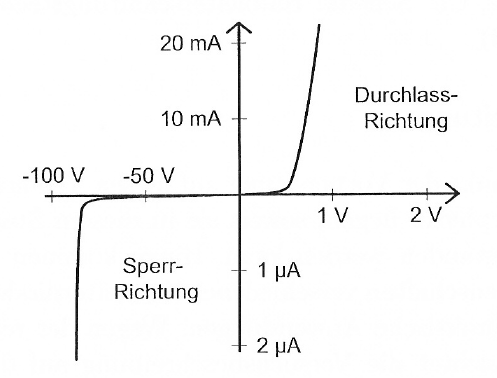
\includegraphics[width=.45\linewidth]{Bilder_aus_Anleitung/2-2.png}
\end{figure}

Dioden können zur Gleichrichtung benutzt werden. Dabei kann die untere
Halbwelle blockiert werden, oder mit einem Zweiweggleichrichter auch die untere
Halbwelle zu einer positiven Spannung umgewandelt werden. Siehe Abbildung
\ref{fig:2.4}. Mit einem Glättungskondensator kann diese $|\sin(\omega t)|$
Spannung, noch zu einer besseren Gleichspannung mit weniger Restwelligkeit
gemacht werden.

\begin{figure}[h]
	\centering
	\caption{%
		Ein- und Zweiweggleichrichter \cite[Abbildung~2.4]{physik313-Anleitung}
	}
	\label{fig:2.4}
	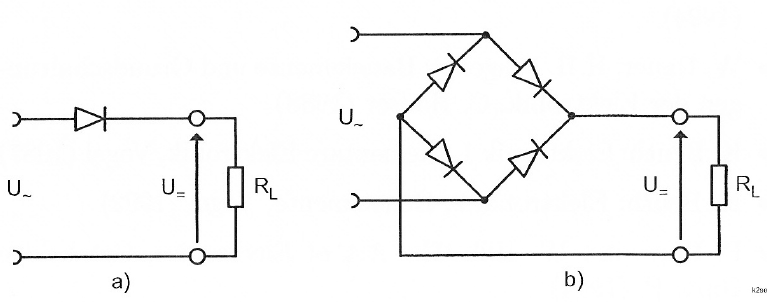
\includegraphics[width=.7\linewidth]{Bilder_aus_Anleitung/2-4.png}
\end{figure}

Mit einer Zenerdiode kann ein Stromteiler aufgebaut werden, der die
Lastspannung stabilisiert. So können stabilisierte Netzteile gebaut werden.

Für die dynamische Messung der Kennlinien benutzen wir das Oszilloskop. Da es
nur Spannungen anzeigen kann, wandeln wir den Strom mit einem Ohm'schen
Widerstand in eine Spannung um. So kann im $x$-$y$-Betrieb direkt die Kennlinie
sichtbar gemacht werden, wenn das System von einem Sägezahn angetrieben wird.

%%%%%%%%%%%%%%%%%%%%%%%%%%%%%%%%%%%%%%%%%%%%%%%%%%%%%%%%%%%%%%%%%%%%%%%%%%%%%%%
%                                  Aufgaben                                   %
%%%%%%%%%%%%%%%%%%%%%%%%%%%%%%%%%%%%%%%%%%%%%%%%%%%%%%%%%%%%%%%%%%%%%%%%%%%%%%%

\section{Aufgaben}

\subsection{Aufgabe A}

\begin{problem}
	Wieviele Energieniveaus gibt es in den erlaubten Bändern des Bändermodells?
\end{problem}

Bei Silizium gibt es 4 Zustände im Valenzband, keine in der Bandlücke und 4 im
Leitungsband. \cite[Vorlesung~16, Folie~13]{meschede/physik441}

\subsection{Aufgabe B}

Dotierung benutzt man, um freie Ladungsträger zu erhalten. In Halbleitern wäre
sonst kein Zustand im Leitungsband besetzt. Dies erreicht man, in dem man Atome
mit anderer Wertigkeit an Kristallplätze setzt und Si so ersetzt. Dies ist eine
gezielte Verunreinigung.

\subsection{Aufgabe C}

\begin{quote}
	Was sind Donatoren und Akzeptoren?
\end{quote}

Beides sind Atome mit anderer Wertigkeit als die umgebenen Kristallatome. Zum
Beispiel P oder B in einem Si- oder Ge-Gitter. Bei P sind reichen die
Valenzelektronen für die Bindungen zu den Nachbarn aus, es bleibt jedoch noch
ein Elektron übrig, das nur mit einer kleinen Ionisationsenergie an den Kern
gebunden ist. So wird der Kristall einfach leitend.

Donatoren und Akzeptoren bringen also ein zusätzliches, freies Elektron bzw.
Loch in den Kristall. \cite[§~18.4.2]{meschede-gerthsen_24}

\subsection{Aufgabe D}

In \cite[§~6.1]{schenke/bauelemente} ist folgende Formel gegeben. Dabei ist
$C_\text S$ die Kapazität der Sperrschicht, $\varepsilon$ die
Dielektrizitätszahl und $d$ die Schichtdicke:
\[
	C_\text S = \frac{\varepsilon A}d
\]

Dies kann nach der Schichtdicke $d$ aufgelöst werden. Wenn man die anderen
Größen messen kann, hat man die Schichtdicke.

\subsection{Aufgabe E}

Sie verändert sich nichtlinear. \cite[§~15.2.2]{beuth/elementare_elektronik}

Mit der Diffusionsspannung $U_\text D$ und $n$ von den physikalischen
Eigenschaften der Diode abhängig:
\cite[§~1.1.1.1.2]{antula/schaltungen_mikroelektronik}
\[
	C_R = \frac{C_0}{\del{1- \frac U{U_\text D}}^n}
\]

\subsection{Aufgabe F}

\subsubsection{Einfacher Widerstand}

Beim einfachen Widerstand $R$ gilt:
\[
	I = \frac 1R U
\]

Dies ist in Abbildung \ref{fig:F-Widerstand} skizziert.

\begin{figure}[h]
	\centering
	\caption{%
		Kennlinie des Ohm'schen Widerstands
	}
	\label{fig:F-Widerstand}
	\includegraphics{Zeichnungen/F-Widerstand.pdf}
\end{figure}

\subsubsection{Einfache Diode}

Für die Diode gilt die in Abbildung 2.2 der Aufgabenstellung gezeichnete
Kennlinie, ich habe sie in Abbildung \ref{fig:F-Diode} selbst gemalt.

\begin{figure}[h]
	\centering
	\caption{%
		Kennlinie der einfachen Diode
	}
	\label{fig:F-Diode}
	\includegraphics{Zeichnungen/F-Diode.pdf}
\end{figure}

\subsubsection{Diode und Widerstand seriell}

Hier gibt die Diode den Stromverlauf vor. Der Widerstand verschlingt jedoch
noch Spannung, wenn Strom fließt. Somit hat die Diode weniger Spannung, es
fließt weniger Strom. Darauf fällt weniger Spannung über dem Widerstand ab, die
Diode hat mehr spannung zur Verfügung. Wir haben versucht, die analytisch zu
lösen, sind jedoch nur anschaulich weitergekommen.

So haben wir uns überlegt, dass der Durchlass erst bei höherer Spannung
einsetzt und dann flacher einsteigt. Dies ist in Abbildung \ref{fig:F-seriell}
skizziert.

\begin{figure}[h]
	\centering
	\caption{%
		Kennlinie der Reihenschaltung
	}
	\label{fig:F-seriell}
	\includegraphics{Zeichnungen/F-seriell.pdf}
\end{figure}

\subsubsection{Diode und Widerstand parallel}

Hier liegt die gleiche Spannung an Diode und Widerstand an. Die Leitfähigkeiten
addieren sich:
\begin{align*}
	Y_\text{ext} &= Y_\text D + Y_R \\
	I_\text{ext} &= (Y_\text D + Y_R) U \\
	&= \del{\frac{f_\text D(U)}U + \frac 1R} U \\
	&= f_\text D (U) + \frac UR \\
	&= f_\text D (U) + f_R(U) \\
	&= (f_\text D + f_R)(U)
\end{align*}

Somit summieren sich beide Kennlinien auf, siehe Abbildung
\ref{fig:F-parallel}.

\begin{figure}[h]
	\centering
	\caption{%
		Kennlinie der Parallelschaltung
	}
	\label{fig:F-parallel}
	\includegraphics{Zeichnungen/F-parallel.pdf}
\end{figure}

\subsubsection{Ideale Spannungsquelle}

Eine ideale Spannungsquelle mit eingestellter Spannung $U_0$ hat einen
Innenwiderstand $R_\text i$. Wenn man die Quelle kurzschließt, fließt der
Strom:
\[
	I = \frac{U_0}{R_\text i}
\]

Wir noch eine externe Spannung angelegt, fließt mehr oder weniger Strom durch
den Innenwiderstand:
\[
	I = \frac{1}{R_\text i} (U_0 + U_\text{ext})
\]

Dies ist in Abbildung \ref{fig:F-Spannungsquelle} skizziert.

\begin{figure}[h]
	\centering
	\caption{%
		Kennlinie der idealen Spannungsquelle
	}
	\label{fig:F-Spannungsquelle}
	\includegraphics{Zeichnungen/F-Spannungsquelle.pdf}
\end{figure}

\subsubsection{Ideale Stromquelle}

Die ideale Stromquelle hat einen Innenwiderstand $R_\text i$, die Quelle passt
die Spannung aber so an, dass der einstellte Strom $I_0$ fließt. Wenn extern
Spannung $U$ angelegt wird, hat die Stromquelle nur mehr oder weniger zu tun,
der Strom fließt trotzdem.
\[
	I = I_0
\]

Dies haben wir in Abbildung \ref{fig:F-Stromquelle} skizziert.

\begin{figure}[h]
	\centering
	\caption{%
		Kennlinie der idealen Stromquelle
	}
	\label{fig:F-Stromquelle}
	\includegraphics{Zeichnungen/F-Stromquelle.pdf}
\end{figure}

\subsection{Aufgabe G}

Die eingehende Wechselspannung wird unten abgeschnitten. Da die
Eingangsspannung weit über der Durchlassspannung ist, wird unten nichts
nennenswertes abgeschnitten. Es ergibt sich ein Spannungsverlauf wie in
Abbildung \ref{fig:G-einfach}.

\begin{figure}[h]
	\centering
	\caption{%
		Spannungsverlauf nach der einfachen Gleichrichtung
	}
	\label{fig:G-einfach}
	\includegraphics{Zeichnungen/G-einfach}
\end{figure}

Bei der zweiten Schaltung wird auch die untere Halbwelle durchgelassen,
allerdings nach oben geklappt. Es kommt zu einem Spannungsverlauf wie in
Abbildung \ref{fig:G-doppelt}.

\begin{figure}[h]
	\centering
	\caption{%
		Spannungsverlauf nach der doppelten Gleichrichtung
	}
	\label{fig:G-doppelt}
	\includegraphics{Zeichnungen/G-doppelt.pdf}
\end{figure}

\subsection{Aufgabe H}

Der Kondensator sollte so groß sein, dass die Kapazität sich in einem Zyklus
nicht komplett entlädt.

Angenommen, das Signal ist ein Rechteck mit Periode T. Dann ist die
Zeitkonstante des Kondensators $\tau = R_\text L C$. Es sollte $\tau \gg T$
gelten. Somit ist $C \gg T R_\text L$.

Wenn $C \to \infty$ geht, muss der Kondensator immer länger aufladen, bis er
die Durchschnittsspannung erreicht hat. Dadurch wird das System träge und zieht
zu beginn beliebig hohe Ströme aus der Diode. Dieser Aspekt wird in einer
späteren Aufgabe noch behandelt.

\subsection{Aufgabe I}

In Abbildung \ref{fig:I-Schaltungen} sind zwei Möglichkeiten zur
Kennlinienmessung dargestellt.

\begin{figure}[h]
	\centering
	\caption{%
		Mögliche Schaltungen zur Kennlinienmessung
	}
	\label{fig:I-Schaltungen}
	\includegraphics{Zeichnungen/I-Schaltungen.pdf}
\end{figure}

Schaltung \textcircled 1 hat den Vorteil, dass nur die Spannung, die an der
Diode abfällt gemessen wird. Schaltung \textcircled 2 hat den Vorteil, dass nur
der Strom, der durch die Diode geht, gemessen wird. Der Strom, der durch den
Spannungsmesser geht, wird nicht gemessen.

In \cite[Bild 14.2]{beuth/elementare_elektronik} ist einfach nur Schaltung
\textcircled 1 als „Schaltung zur Aufnahme der Diodenkennlinien $I = f(U)$“
dargestellt.

So ist es wahrscheinlich am sinnvollsten, Schaltung \textcircled 1 für beide
Messungen zu benutzen. Da bei der Sperrung kleine Ströme fließen, allerdings
hohe Spannungen auftreten, ist es vielleicht sinnvoll, dafür \textcircled 2 zu
benutzen, um den Strommessfehler durch den Innenwiderstand des Spannungsmessers
zu vermeiden.

\subsection{Aufgabe J}

Man lässt den Strom durch einen Ohm'schen Widerstand laufen, an diesem fällt
dann eine zum Strom proportionale Spannung ab.

Dies erfährt man auch, wenn man etwas weiter ließt und sich Abbildung 2.7 aus
der Anleitung anschaut.

\subsection{Aufgabe K}

Der maximale Durchlassstrom ist \SI{1000}{\milli\ampere}. Wenn $C$ zu groß ist,
zieht $C$ zu viel Strom. In $\Deltaup t := \SI{100}{\micro\second}$ geht die
Spannung um $\Deltaup U := \SI1\volt$ hoch. Die Ladungszunahme ist $\Deltaup Q
= C \Deltaup U$.

Der Strom ist:
\[
	I = \frac{\Deltaup Q}{\Deltaup t}
	= C \frac{\Deltaup U}{\Deltaup t}
\]

Dies muss kleiner als $I_\text{max}$ sein:
\[
	I_\text{max} \frac{\Deltaup t}{\Deltaup U} > C
	\implies
	C < \SI{100}{\micro\farad}
\]

\subsection{Aufgabe L}

Wenn die Wechselspannungsquelle gerade ganz negativ ist, so wirkt auf die Diode
einmal die Spannung $- U_0$ von der Spannungsquelle. Außerdem wird noch einmal
eine Spannung $-U_0$ durch den Kondensator auf die Diode. Es liegen also
$-2U_0$ an.

\subsection{Aufgabe M}

\subsubsection{Schaltung a}

Unterhalb der Sperrspannung kann hier kein Strom fließen. Die Ausgangsspannung
ist quasi identisch null.

\subsubsection{Schaltung b}

Hier kann Strom fließen, allerdings macht die diagonale Diode nichts. Dies ist
ein einfacher Gleichrichter, der Ausgabestrom ist der gleiche wie in Abbildung
\ref{fig:G-einfach}.

\subsubsection{Schaltung c}

Dies ist nur eine andere Darstellung von Schaltung b, so dass die gleichen
Überlegungen auch hier zutreffen. Die Umformung ist in Abbildung
\ref{fig:M-Schaltung_drei} dargestellt.

\begin{figure}[h]
	\centering
	\caption{%
		Umformung von Schaltung c
	}
	\label{fig:M-Schaltung_drei}
	\includegraphics{Zeichnungen/M-Schaltung_drei.pdf}
\end{figure}

\subsection{Aufgabe N}

$U'$ ist die Spannung an der Last. Der Gesamtstrom, der fließt ist:
\[
	I = \frac{U_0}{R + R_\text L}
\]

\newcommand\RL{R_\text L}

Die Spannung $U'$ ist:
\begin{align*}
	U'
	&= \RL I \\
	&= \RL \frac{U_0}{R + R_\text L} \\
	&= \frac{U_0 \RL}{R + \RL} \\
	&+ \frac{U_0}{1 + \frac R\RL}
\end{align*}

Die Funktion ist in Abbildung \ref{fig:N-Plot} skizziert.

\begin{figure}[h]
	\centering
	\caption{%
		Lastspannung in Abhängigkeit vom Lastwiderstand
	}
	\label{fig:N-Plot}
	\includegraphics{Zeichnungen/N-Plot.pdf}
\end{figure}

Die Extremwerte sind $I = U/R$, wenn $\RL = 0$ sowie $U' = U_0$ wenn $\RL \to
\infty$.

\subsection{Aufgabe O}

\newcommand\IZmax{I_\text{Z,max}}
\newcommand\IZmin{I_\text{Z,min}}
\newcommand\IZ{I_\text Z}
\newcommand\UZ{U_\text Z}

Der Strom $\IZmax$ darf nicht überschritten werden. Mit dem Ansatz aus 
\cite[§~15.1.3]{beuth/elementare_elektronik} betrachte ich zuerst $\RL =
\infty$. Dann fällt an der Zenerdiode gerade $\UZ$ ab, über $R$ fällt $U - \UZ$
ab. Damit der Strom nicht überschritten wird, muss gelten:
\[
	R > \frac{U - \UZ}\IZmax
\]

Diese Bedingung ist erfüllt:
%\[
	%\SI{200}\ohm > \frac{\SI{8.2}\volt}{\SI{100}{\milli\ampere}} = \SI{82}\ohm
%\]

Der extremste Fall tritt ein, wenn $U$ maximal wird. Also ist die untere
Schranke für $R$:
\[
	R > \frac{\SI{22}\volt - \SI{8.2}\volt}{\SI{100}{\milli\ampere}}
	= \SI{138}\ohm
\]

Dies ist die untere Grenze. Wenn weniger als $\IZmin$ durch die Zenerdiode
fließen, ist die STabilisierung auch weg. Also im unbelasteten Fall:
\[
	\frac U\IZmin > R
\]

Nehme minimales $U$ für Extremwert:
\[
	R < \SI{8}{\kilo\ohm}
\]

Wenn jetzt die Last dazukommt, wird der Zenerstrom allerdings kleiner. Sobald
dann jedoch die Spannung wieder ansteigt, sollte der Zenerstrom wieder groß
genug werden.

Somit ist der Bereich \SIrange{138}{8000}{\ohm}.

%%%%%%%%%%%%%%%%%%%%%%%%%%%%%%%%%%%%%%%%%%%%%%%%%%%%%%%%%%%%%%%%%%%%%%%%%%%%%%%
%                      Versuchsaufbau und -durchführung                      %
%%%%%%%%%%%%%%%%%%%%%%%%%%%%%%%%%%%%%%%%%%%%%%%%%%%%%%%%%%%%%%%%%%%%%%%%%%%%%%%

\section{Versuchsaufbau und -durchführung}

%%%%%%%%%%%%%%%%%%%%%%%%%%%%%%%%%%%%%%%%%%%%%%%%%%%%%%%%%%%%%%%%%%%%%%%%%%%%%%%
%                                 Auswertung                                  %
%%%%%%%%%%%%%%%%%%%%%%%%%%%%%%%%%%%%%%%%%%%%%%%%%%%%%%%%%%%%%%%%%%%%%%%%%%%%%%%

\section{Auswertung}

%%%%%%%%%%%%%%%%%%%%%%%%%%%%%%%%%%%%%%%%%%%%%%%%%%%%%%%%%%%%%%%%%%%%%%%%%%%%%%%
%                                  Ergebnis                                   %
%%%%%%%%%%%%%%%%%%%%%%%%%%%%%%%%%%%%%%%%%%%%%%%%%%%%%%%%%%%%%%%%%%%%%%%%%%%%%%%

\section{Ergebnis}

\IfFileExists{\bibliographyfile}{
	\bibliography{\bibliographyfile}
}{}

\end{document}

% vim: spell spelllang=de
